\section{Sobre redes neuronales}
  \blindtext
\subsection{Descenso por el gradiente}
Uno de los puntos clave del aprendizaje de máquina supervisado es
definir una función objetivo que deberá ser optimizada durante el
proceso de aprendizaje. Esta función objetivo usualmente es una
\textbf{función de costo, pérdida o error} que se quiere minimizar.

Definimos la función de costo $J$ como la \textbf{Suma de los errores
  cuadrados (SSE)} entre la salida calculada y el valor real.
\begin{equation}
  J(w)=1/2n \sum_i (\hat{y}_i - y_i^2)
\end{equation}
donde $w$ es el conjunto de los parámteros de la red, es decir $w :=
\bigcup{W_i, b_i}_{i=1}^{n}$, $n$ el número de capas de la red, y
$y_i$ la $i$-ésima etiqueta de entrenamiento. La principal ventaja de
esta función de error, además de ser lineal es que la función de
costos se vuelve diferenciable.

La no-linealidad de las funciones de activación provoca que no se
garantice la convexidad de las funciones de error más comunes, es
decir, que no existe un método analítico para encontrar el mínimo de
la función de error. El entrenamiento de la red se basa en métodos
iterativos que van reduciendo paulatinamente ese error.

Sabemos que la derivada es útil para minimizar funciones porque, dada
una función $y = f(x)$, nos dice cómo cambiar $x$ para hacer una
pequeña mejora en $y$, en otras palabras $f(x-\varepsilon f'(x)) <
f(x)$ para un $\varepsilon \in \mathbb{R}$ suficientemente
pequeño. Podemos entonces minimizar $f(x)$ al mover a $x$ en pequeños
\textit{pasos} con el signo opuesto de la derivada. A esta técnica se
le conoce como \textbf{descenso por el gradiente}.

La idea detrás del descenso por el gradiente es disminuir el gradiente hasta encontrar
un mínimo (local o global) de la función de costo. En cada iteración, se reduce
un \textit{paso} del gradiente, donde cada \textit{paso} está determinado por
el valor del índice de aprendizaje, así como por la pendiente del gradiente.

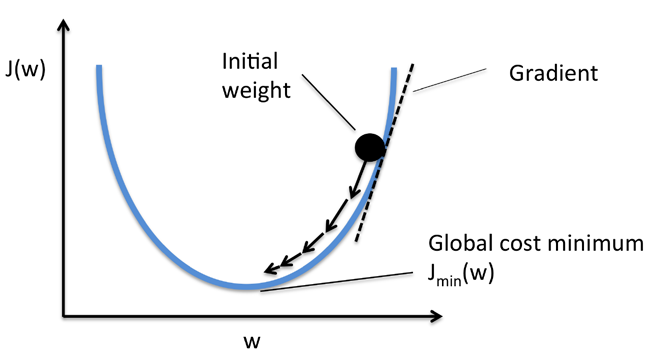
\includegraphics[scale=0.5]{gradient-descent}

Usando el descenso por el gradiente, se pueden actualizar los pesos quitandole un \textit{paso}
al gradiente $\nabla J(w)$ de la función de costos $J(w)$:
\begin{equation}
  w := w + \Delta w
\end{equation}

En donde el cambio de peso $\Delta w$ se define como el gradiente negativo multiplicado
por el índice de aprendizaje $\eta$:
\begin{equation}
  \Delta w := -\eta \Delta J(w)
\end{equation}

Calculamos la derivada parcial de la función de costos SSE con respecto al
j-ésimo peso de la siguiente manera:
\begin{equation*}
\begin{split}
  \frac{\partial J}{\partial w_j} &= \frac{\partial}{\partial w_j}\frac{1}{2}\sum_i (y^{(i)} - \phi(z^{(i)}))^2 \\
  &= \frac{1}{2}\sum_i 2(y^{(i)} - \phi(z^{(i)}))\frac{\partial}{\partial w_j}(y^{(i)} - \phi(z^{(i)}))\\
  &= \sum_i (y^{(i)} - \phi(z^{(i)}))\frac{\partial}{\partial w_j}(y^{(i)} - \phi (z^{(i)}))\\
  &= \sum_i(y^{(i)} - \phi(z^{(i)}))(-x_j^{(i)})\\
  &= -\sum_i(y^{(i)} - \phi(z^{(i)}))x_j^{(i)}
\end{split}
\end{equation*}

Las redes neuronales (ANN por sus siglas en inglés) son modelos
complejos que por lo general tienen un alto número de mínimos locales,
volviendo al descenso por el gradiente poco efectivo como mecanismo de
entrenamiento.  Sin embargo, redes altamente eficientes por lo general
son entrenadas utilizando descenso por el gradiente. ¿Cómo explicar
esta aparente contradicción?

Recientemente, evidencia empírica \cite{choromanska} ha dado indicios
de que las ANN tienen la mayoría de sus mínimos locales cerca del
mínimo global.  Esto quiere decir que \textbf{el descenso por el
  gradiente funciona ``suficientemente bien''}. Hay otros métodos más
avanzados que son empleados para entrenar ANNs, pero este trabajo
utiliza descenso por el gradiente por su simplicidad e interpetación
tan intuitiva.

\subsection{Propagación hacia atrás}
FALTA SECCIÓN
\cite{haykin} 129
\cite{memes} 36
http://www.iro.umontreal.ca/~pift6266/H10/notes/mlp.html

\subsection{Convolución}
FALTA SECCIÓN
